  I risultati ottenuti sono riassunti in Fig.\ref{fig:dati-raw}.
  I parametri risultanti dal \emph{fit} sono riassunti in Tab.\ref{tab:risultati-fit}.
  I fit sono stati svolti usando l'algoritmo \emph{Gradient}\footnote{https://reference.wolfram.com/language/ref/NonlinearModelFit.html} di \emph{Woflram Mathematica}\footnote{https://www.wolfram.com/mathematica/}, e le rispettive incertezze %todo add ref
  sono date dagli errori standard dei parametri ottenuti dal \emph{fit}.                                          %todo add ref
  Qualitativamente, l'andamento è concorde con quanto atteso. In Fig.\ref{fig:raw-pi}
  si vede chiaramente che la funzione raggiunge lo zero per un certo angolo $\theta$,
  mentre in Fig.\ref{fig:raw-sigma} la funzione cresce monotonamente.
  %\footnote{In realtà nella nostra implementazione il valore di $V_{sig}$ è
  %  moltiplicato per una costante $k = (1024 \cdot 5)^{-1 V^{-1}}$, in modo
  %  da ottenere un intervallo di valori in uscita compreso in un range tra $0$ e
  %  $1000$.}
  \begin{figure}[H]
    \centering
    \caption{Dati raccolti}
    \begin{subfigure}[t]{.4\textwidth}
      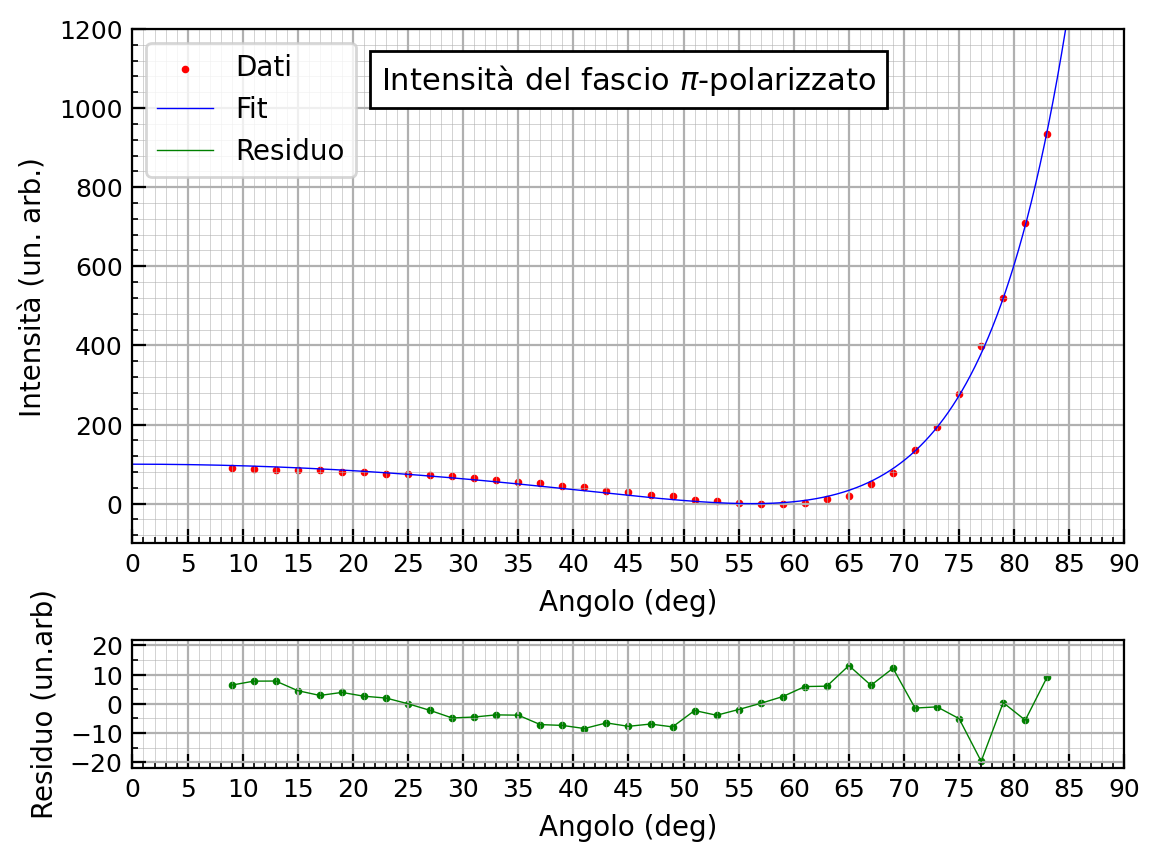
\includegraphics[width=7cm]{./graphs/raw-pi.png}
      \caption{
        \emph{
          Dati di intensità luminosa con luce polarizzata perpendicolarmente al
          piano di incidenza e relativo fit. Dal grafico si vede chiaramente che
          l'intensità luminosa si annulla per un certo valore di $\theta_i$.
        }
      }
      \label{fig:raw-pi}
    \end{subfigure}
    %
    \hspace{20mm}
    %
    \begin{subfigure}[t]{.4\textwidth}
      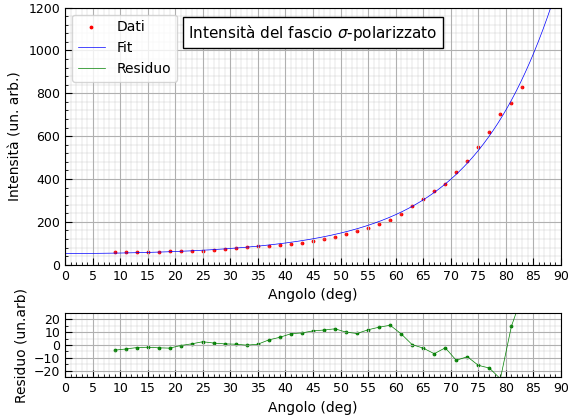
\includegraphics[width=7cm]{./graphs/raw-sigma.png}
      \caption{
        \emph{
          Dati di intensità luminosa con luce polarizzata parallelamente al
          piano di incidenza e relativo fit.
        }
      }
      \label{fig:raw-sigma}
    \end{subfigure}
    \label{fig:dati-raw}
  \end{figure}
  %
  \begin{table}[ht]
    \centering
    \caption{Risultati dei \emph{fit} dei dati raccolti}
    \begin{tabular}[t]{cc}
      \toprule
      Parametro &Valore ottenuto\\
      \midrule
      $I_{0\pi}$    &??? \\ %todo
      $I_{0\sigma}$ &??? \\ %todo
      $n_{2\pi}$ &??? \\ %todo
      $n_{2\sigma}$ &??? \\ %todo
      \bottomrule
    \end{tabular}\label{tab:risultati-fit}
  \end{table}
  %
  Abbiamo misurato valori nell'intervallo di ${\theta_{min} \leq \theta \leq \theta_{max}}$,
  con ${\theta_{min} = 7^\circ \pm 0.5^\circ}$ e ${\theta_{max} = 83^\circ \pm 0.5^\circ}$.
  Le dimensioni del lato del prisma utilizzato ($15mm$ di lunghezza) non permettevano
  di andare oltre $\theta_{max}$ senza che il fascio venisse alterato, mentre il
  limite di $\theta_{min}$ ci è stato imposto dalla geometria del sensore.
  Abbiamo scelto un passo angolare di $2^\circ$ per permetterci di prendere un
  numero adeguato di misure, senza allungare eccessivamente la durata dell'esperimento.
  Il campione di dati riportato in Fig.\ref{fig:dati-raw} è quello che segue meglio
  l'andamento previsto.
  Le incertezze associate ad ogni punto sono state ottenute come somma somma di
  incertezze sistematiche dovute all'attrezzatura e di incertezze casuali, come
  descritto in Sez.\ref{subsec:calcolo-incertezza-strumentale} e Sez.\ref{subsec:calcolo-incertezza-casuale}.

  Normalizzando i dati, si ottengono i risultati mostrati in Fig.\ref{fig:normalised-coefficients} %todo capire se per normalizzare basta dividere per I_0, o se conviene imporre anche che i due n2 siano uguali.
                                                                    %  ceh in realtà ci sta prenderne la media per soddisfare a condizione di Lipson.
  assieme all'andamento previsto\footnote{Calcolato supponendo di avere un valore di $n_2 = 1.519$,%todo expand me
  caratteristico per il vetro K9 alla lunghezza della luce rossa.}.
  %
  \begin{figure}[H]
    \centering
    \caption{Smegma}
    \begin{subfigure}{.4\textwidth}
      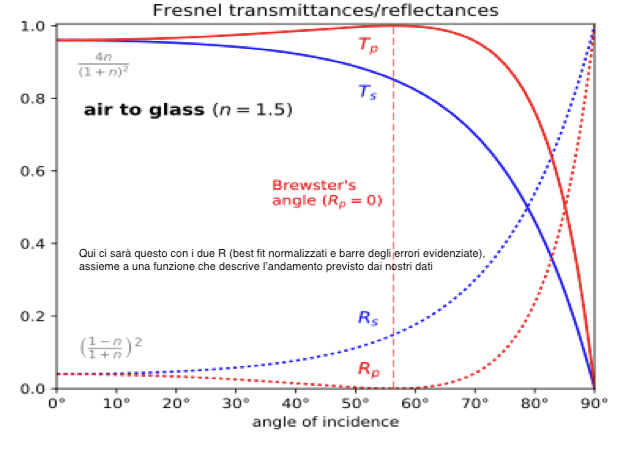
\includegraphics[width=7cm]{./graphs/normalised-coefficients.png}
      \caption{
        \emph{
          spregna
        }
      }
      \label{fig:normalised-coefficients}
    \end{subfigure}%
    \hspace{20mm}
    \begin{subfigure}{.4\textwidth}
      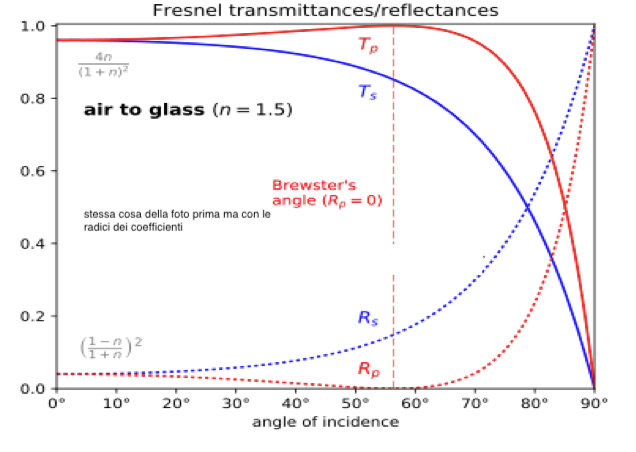
\includegraphics[width=7cm]{./graphs/amplitude-coefficients.png}
      \caption{
        \emph{
          bora
        }
      }
      \label{fig:coefficienti-ampiezza}
    \end{subfigure}
  \end{figure}
%
\subsection{Misura dell'angolo di Brewster}\label{subsec:angolo-di-brewster}
  Inserendo nell'equazione \eqref{legge-brewster} $n_1 = 1.000$ e $n_2 = ???$ %todo add
  otteniamo un valore per l'angolo di Brewster $\theta_B = ??? \pm ????$. Il valore di $n_2$ utilizzato è la media
  dei due coefficienti in Tab.\ref{tab:risultati-fit}.
  Possiamo ottenere un'altra stima per $\theta_B$ con un \emph{fit} parabolico nella stretta regione
  dove $R_\pi$ si annulla; il vertice della parabola è la miglior stima per $\theta_B$.
  Il risultato ottenuto è $\theta_B = ???$, ed è mostrato in figura \ref{fig:brewsters-angle}. %todo add
  %
  \begin{figure}[h]
    \centering
    \caption{brema}
    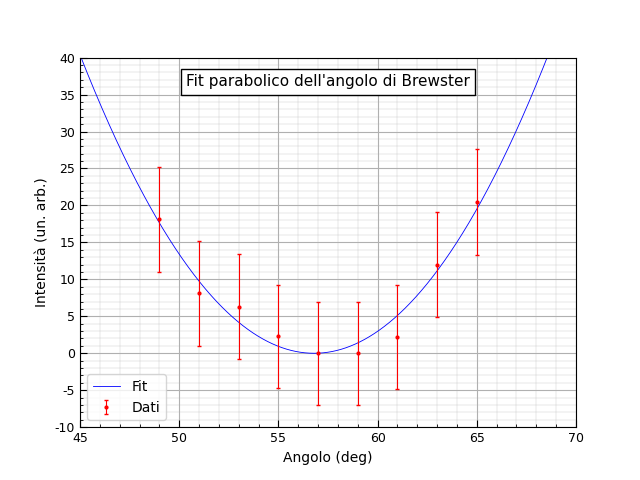
\includegraphics[width=7cm]{./graphs/brewsters-angle.png}
    \label{fig:brewsters-angle}
  \end{figure}
  % TODO
\endinput



